\section{\textit{Supplementary Material for \cref{subsec:scaling}: Results -- Runtime and Performance Scaling}}
\label{app:runtime_details}


\subsection{Experimental Details}

\paragraph{Grids and sample counts.}
We evaluate small IEEE~14/30/57/118 and large GOC~500/2{,}000/10{,}000 grids. All solvers process the same number of instances per network, respectively:
\[
4\times10^{6},\;
3\times10^{6},\;
2\times10^{6},\;
2\times10^{6},\;
5\times10^{5},\;
5\times10^{4},\;
10^{4}.
\]
Each benchmark run at the selected optimal batch size lasts approximately 20\,s or longer, making initialization operations a small fraction of the measured runtime while keeping the full search for the best batch size or number of workers tractable (runs with suboptimal batch sizes or worker counts can take much longer). All runtime experiments consumed 37.5 H100 GPU-hours for \genco and 343 CPU-node-hours for the PowerModels-based classical solvers.

\paragraph{\genco.}
Inference uses FP32 GPU execution with \texttt{torch.compile(mode="reduce-overhead")}. Each job uses one exclusive H100 80\,GB GPU, 40 CPU cores, and 128\,GB of host RAM; this was sufficient because only $10^4$ samples are resident in memory at once. Batch sizes are powers of two from 64 to 16{,}384 on IEEE grids and from 16 to 16{,}384 on GOC grids. Inference uses 32 DataLoader workers.

\paragraph{Classical solvers implemented through PowerModels.}
AC-PF uses PowerModels' NLsolve-based Newton solver through GOC~500 and a more robust JuMP model on GOC~2{,}000/10{,}000. AC-OPF and DC-OPF use IPOPT with MUMPS; IPOPT uses tolerance $10^{-6}$ and \texttt{max\_iter}=100. Each job is assigned all 84 physical CPU cores of one node, with one Basic Linear Algebra Subprogram (BLAS) thread per worker. The worker sweep is $p\in\{24,40,\ldots,216\}$ (with increments of 16). Reproducing the experiments requires at least 256\,GB for small grids and 960\,GB for large grids. Dispatch batch size is 32 (workers get 32 scenarios to solve at once) on small grids and 1 on large grids to amortize scheduling overhead where solves are cheap without delaying dynamic load balancing on expensive cases.


\subsection{Batch-Size and Worker-Count Sweeps}
\label{appendix:sweep}

\genco's wall-clock time per instance versus batch size for all grids and Base/Small/Tiny models is depicted in \cref{fig:batchsize_vs_runtime_appendix}. Wall-clock time per instance versus worker count for the PowerModels-based classical solvers is shown in \cref{fig:workers_vs_runtime_appendix}. Larger batches or worker pools reduce wall-clock time per instance until saturation; larger models and grids saturate earlier.

\begin{figure}[H]
    \centering
    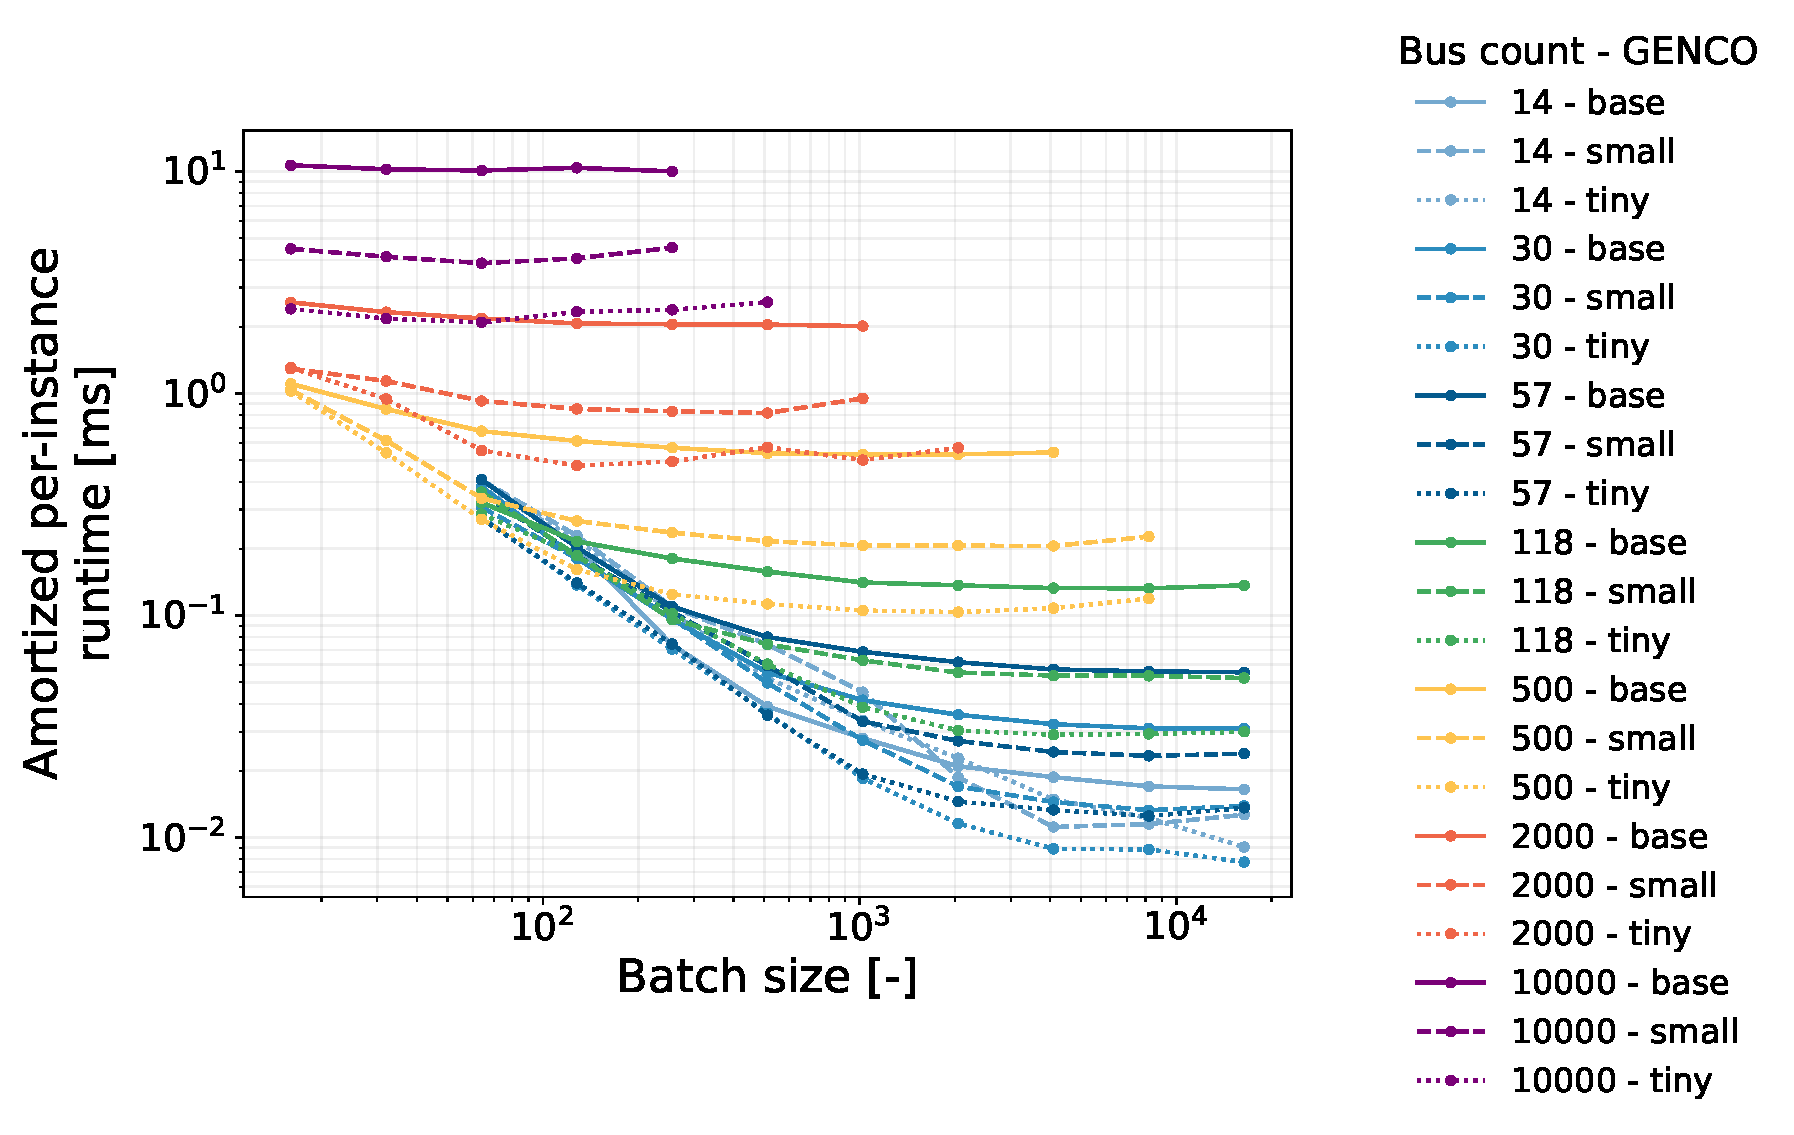
\includegraphics[width=0.5\columnwidth]{figures/runtime_analysis/pf_opf_benchmark_matrix_appendix.pdf}
    \caption{\genco wall-clock time per instance versus batch size across grids and model scales.}
    \label{fig:batchsize_vs_runtime_appendix}
\end{figure}

\begin{figure}[H]
    \centering
    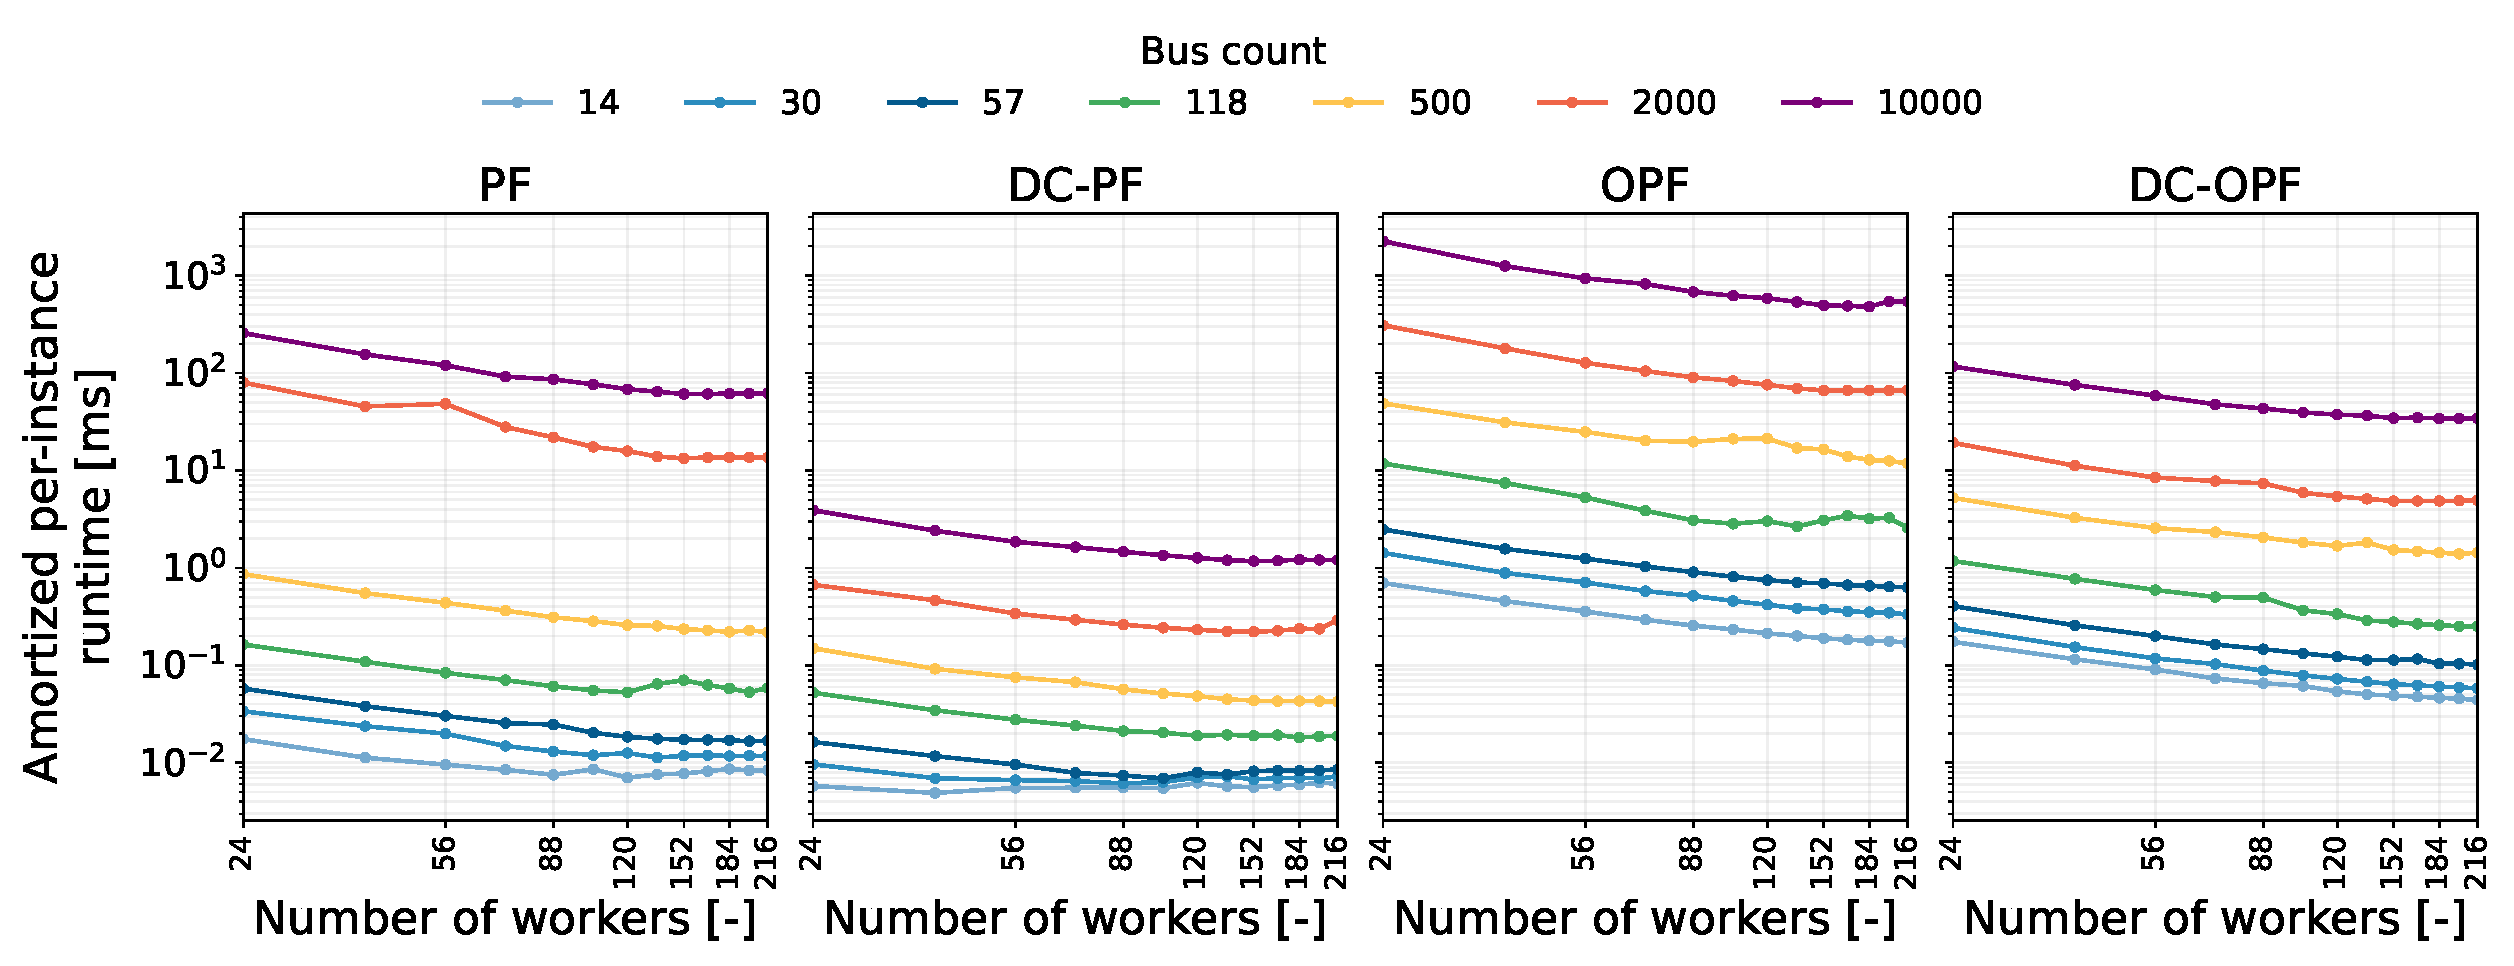
\includegraphics[width=0.7\columnwidth]{figures/runtime_analysis/juliacall_scaling_comparison.pdf}
    \caption{Wall-clock time per instance versus worker count for the PowerModels-based classical AC-PF, DC-PF, AC-OPF, and DC-OPF solvers across grids using the in-memory protocol.}
    \label{fig:workers_vs_runtime_appendix}
\end{figure}


\subsection{Runtime Analysis With and Without Data Loading}
\label{app:s1_vs_s2}

\paragraph{Protocols.}

The main results in \cref{subsec:scaling} use an \emph{in-memory protocol} designed to represent repeated scenario analysis around a reference operating point. The \emph{from-disk protocol} complements this setup by considering grid snapshots in which each scenario is an independent input loaded from disk. The two protocols therefore capture two distinct use cases: repeated in-memory perturbations around a base operating point, and solving heterogeneous scenarios retrieved from storage.

\paragraph{Practical differences.}

In the \emph{in-memory protocol}, both solver classes use preprocessed, parsed, and memory-resident scenarios: GENCO cycles over $10^4$ already loaded tensors in RAM, while each PowerModels worker uses an already parsed base case. The number and content of the tensors do not affect solve runtime; the large pool is used only to avoid potential caching effects. In contrast, in the \emph{from-disk protocol}, both solver classes read scenarios from disk: GENCO reads each processed sample, while PowerModels reads and parses a ready-to-solve \datakit scenario. In both protocols, GENCO uses batched GPU inference and the PowerModels-based classical solvers use multiple CPU workers, with the same parallelization strategy used to maximize throughput. The only difference in timing scope between the two protocols is whether scenario data loading is included in the measured runtime.\\

The from-disk protocol additionally introduces practical dependencies that are absent from the in-memory protocol, including storage format (e.g., JSON versus other representations), scenario access order (e.g., sequential versus non-sequential access), page-cache state, filesystem type (e.g., local node storage versus GPFS), and system contention. Finally, the solved scenarios differ between the two protocols: the in-memory protocol repeatedly solves the fixed base case, whereas the from-disk protocol solves distinct \datakit scenarios. The use of distinct \datakit scenarios is intentional: the from-disk protocol is designed to represent workloads in which heterogeneous grid snapshots are independently retrieved and solved, rather than repeated perturbations around a single operating point. The resulting runtime difference therefore reflects both data-loading overhead and differences in scenario difficulty and should be interpreted as a comparison of two workload regimes.




\paragraph{Observed effects.}

Loading primarily affects \genco's small-grid speedups as shown in \cref{tab:loading_speedups}. Under the from-disk protocol, \genco is slower than AC-PF on IEEE~14/30/57, but remains faster than AC-OPF on every grid; the large-grid conclusions are unchanged.\\

\begin{table}[H]
\centering
\scriptsize
\setlength{\tabcolsep}{5pt}
\caption{\genco Tiny speedups relative to classical AC-PF and AC-OPF solvers. Speedup is classical solvers' wall-clock time per instance divided by \genco wall-clock time per instance; values above one favor \genco.}
\label{tab:loading_speedups}
\begin{tabular}{@{}l cc cc@{}}
\toprule
& \multicolumn{2}{c}{vs.\ AC-PF} & \multicolumn{2}{c}{vs.\ AC-OPF} \\
\cmidrule(lr){2-3}\cmidrule(lr){4-5}
Grid & In-memory & From-disk & In-memory & From-disk \\
\midrule
IEEE 14     & $0.8\times$  & $0.3\times$  & $18.9\times$  & $6.4\times$ \\
IEEE 30     & $1.5\times$  & $0.4\times$  & $43.0\times$  & $9.5\times$ \\
IEEE 57     & $1.3\times$  & $0.6\times$  & $50.4\times$  & $16.1\times$ \\
IEEE 118    & $1.8\times$  & $1.4\times$  & $88.4\times$  & $50.6\times$ \\
GOC 500     & $2.1\times$  & $2.6\times$  & $114.0\times$ & $108.9\times$ \\
GOC 2{,}000 & $28.2\times$ & $31.4\times$ & $140.0\times$ & $160.8\times$ \\
GOC 10{,}000 & $29.1\times$ & $28.9\times$ & $229.1\times$ & $243.0\times$ \\
\bottomrule
\end{tabular}
\end{table}

Loading matters most when computation is inexpensive and becomes negligible as model or grid complexity grows as depicted in \cref{fig:loading_overhead_best_config}. For PowerModels, loading affects DC-PF most on large grids because JSON parsing complexity grows faster with grid size than DC-PF solve complexity; AC-PF changes by only about $1.0$--$1.3\times$, while OPF remains near parity because optimization dominates parsing. Ratios below one coincide with lower mean solve times over diverse scenarios than for the repeated base case, indicating that the base load and topology are harder than the average scenario.


\begin{figure}[H]
    \centering
    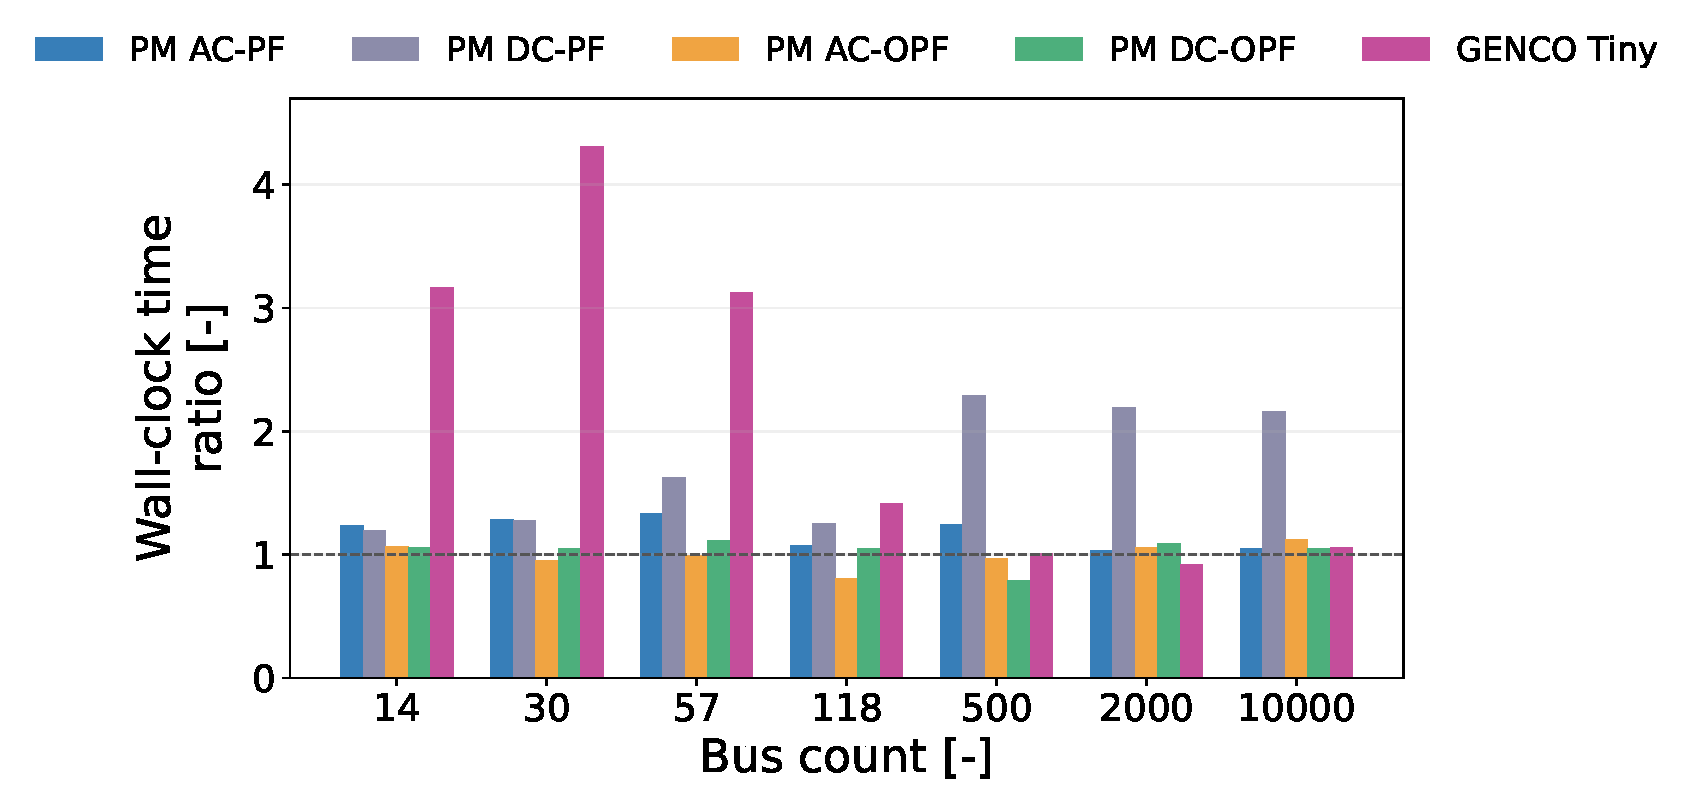
\includegraphics[width=0.5\columnwidth]{figures/runtime_analysis/loading_overhead_best_config.pdf}
    \caption{Ratio of from-disk to in-memory wall-clock time per instance at the best configuration selected independently under each protocol. The dashed line marks equal time; values above one indicate loading overhead.}
    \label{fig:loading_overhead_best_config}
\end{figure}





\subsection{Additional OPF scaling results}

Detailed results for \genco Base and Small from IEEE~14 through GOC~2{,}000 are provided in \cref{tab:opf_scaling}.
\begin{table}[H]
\caption{Constraint violations and optimality gaps for \genco and DC-OPF, with AC-OPF as the optimality reference. Bold entries denote metrics for which the performance difference exceeds one standard deviation. The metrics are computed as described in Section~\ref{subsec:opf}. \genco Base and Small achieve similar feasibility and optimality improvements across all systems.}
\label{tab:opf_scaling}
\centering
\footnotesize
\setlength{\tabcolsep}{4pt}
\begin{tabular}{@{}lllllclll@{}}
\toprule
& & Optimality & \multicolumn{2}{c}{Thermal limits} & \multicolumn{2}{c}{Power balance} & React.\ gen. bounds \\
\cmidrule(lr){3-3}\cmidrule(lr){4-5}\cmidrule(lr){6-7}\cmidrule(lr){8-8}
System & Model
  & Gap (\%)
  & $S_{ij}(+)$ [MVA]
  & $S_{ij}(-)$ [MVA]
  & $\mathrm{PBRes}_{P}$ [MW]
  & $\mathrm{PBRes}_{Q}$ [MVar]
  & $Q_g$ [MVar] \\
\midrule

\multirow{3}{*}{IEEE 14}
  & \genco Base
  & \textbf{0.10 $\pm$ 0.00}
  & 2.56e-5 $\pm$ 1.94e-5
  & 1.32e-5 $\pm$ 2.93e-6
  & \textbf{4.35e-3 $\pm$ 9.46e-5}
  & \textbf{3.79e-3 $\pm$ 1.11e-4}
  & 1.28e-3 $\pm$ 1.57e-4 \\

  & \genco Small
  & 0.10 $\pm$ 0.01
  & 2.46e-5 $\pm$ 1.83e-5
  & 1.37e-5 $\pm$ 2.37e-6
  & 5.51e-3 $\pm$ 5.28e-4
  & 4.63e-3 $\pm$ 6.25e-5
  & \textbf{1.20e-3 $\pm$ 2.44e-4} \\

  & DC-OPF
  & 5.75 $\pm$ 0.01
  & \textbf{0}
  & \textbf{0}
  & 1.42e+0 $\pm$ 4.56e-3
  & --
  & -- \\
\midrule

\multirow{3}{*}{IEEE 30}
  & \genco Base
  & \textbf{0.21 $\pm$ 0.02}
  & 1.13e-3 $\pm$ 1.74e-4
  & \textbf{1.11e-3 $\pm$ 1.55e-4}
  & \textbf{6.90e-3 $\pm$ 1.05e-3}
  & \textbf{4.95e-3 $\pm$ 2.93e-4}
  & \textbf{7.00e-4 $\pm$ 3.11e-4} \\

  & \genco Small
  & 0.25 $\pm$ 0.01
  & \textbf{1.12e-3 $\pm$ 1.94e-4}
  & 1.12e-3 $\pm$ 1.61e-4
  & 1.06e-2 $\pm$ 1.81e-3
  & 8.03e-3 $\pm$ 6.59e-4
  & 8.95e-4 $\pm$ 3.92e-5 \\

  & DC-OPF
  & 7.83 $\pm$ 0.03
  & 9.83e-2 $\pm$ 1.02e-3
  & 7.89e-2 $\pm$ 8.04e-4
  & 6.34e-1 $\pm$ 4.27e-3
  & --
  & -- \\
\midrule

\multirow{3}{*}{IEEE 57}
  & \genco Base
  & 1.21 $\pm$ 0.18
  & 2.89e-3 $\pm$ 3.64e-4
  & 3.04e-3 $\pm$ 6.22e-5
  & 4.13e-1 $\pm$ 1.59e-1
  & 1.80e-1 $\pm$ 7.74e-2
  & \textbf{6.15e-3 $\pm$ 7.11e-4} \\

  & \genco Small
  & \textbf{0.88 $\pm$ 0.14}
  & \textbf{2.69e-3 $\pm$ 5.02e-5}
  & \textbf{2.87e-3 $\pm$ 3.28e-4}
  & \textbf{3.00e-1 $\pm$ 6.92e-2}
  & \textbf{1.62e-1 $\pm$ 3.38e-2}
  & 7.25e-3 $\pm$ 1.28e-3 \\

  & DC-OPF
  & 5.54 $\pm$ 0.02
  & 1.53e-2 $\pm$ 3.36e-4
  & 1.15e-2 $\pm$ 2.26e-4
  & 1.29e+0 $\pm$ 2.51e-3
  & --
  & -- \\
\midrule

\multirow{3}{*}{IEEE 118}
  & \genco Base
  & 1.66 $\pm$ 0.03
  & \textbf{3.75e-2 $\pm$ 5.62e-3}
  & \textbf{3.74e-2 $\pm$ 5.78e-3}
  & 1.36e+0 $\pm$ 1.12e-1
  & 2.75e-1 $\pm$ 2.36e-3
  & 1.19e-3 $\pm$ 6.65e-4 \\

  & \genco Small
  & \textbf{1.66 $\pm$ 0.03}
  & 4.21e-2 $\pm$ 4.48e-5
  & 4.17e-2 $\pm$ 3.73e-4
  & \textbf{1.12e+0 $\pm$ 6.14e-2}
  & \textbf{2.57e-1 $\pm$ 1.49e-2}
  & \textbf{1.13e-3 $\pm$ 1.83e-4} \\

  & DC-OPF
  & 4.73 $\pm$ 0.02
  & 1.04e-1 $\pm$ 6.49e-4
  & 1.06e-1 $\pm$ 6.25e-4
  & 2.46e+0 $\pm$ 3.11e-3
  & --
  & -- \\
\midrule

\multirow{3}{*}{GOC 500}
  & \genco Base
  & \textbf{0.49 $\pm$ 0.08}
  & \textbf{3.83e-3 $\pm$ 3.57e-4}
  & \textbf{3.86e-3 $\pm$ 1.76e-4}
  & \textbf{7.07e-1 $\pm$ 8.16e-2}
  & \textbf{1.89e-1 $\pm$ 2.18e-2}
  & \textbf{4.90e-4 $\pm$ 1.27e-4} \\

  & \genco Small
  & 0.57 $\pm$ 0.01
  & 4.22e-3 $\pm$ 6.91e-6
  & 4.39e-3 $\pm$ 1.76e-4
  & 8.16e-1 $\pm$ 9.95e-3
  & 2.48e-1 $\pm$ 8.65e-3
  & 6.19e-4 $\pm$ 3.00e-5 \\

  & DC-OPF
  & 1.81 $\pm$ 0.01
  & 4.35e-2 $\pm$ 1.47e-4
  & 8.01e-2 $\pm$ 3.20e-5
  & 1.85e+0 $\pm$ 4.12e-3
  & --
  & -- \\
\midrule

\multirow{3}{*}{GOC 2000}
  & \genco Base
  & \textbf{1.53 $\pm$ 0.03}
  & 3.56e-2 $\pm$ 2.35e-2
  & 3.66e-2 $\pm$ 2.49e-2
  & 2.94e+0 $\pm$ 3.05e-1
  & \textbf{7.93e-1 $\pm$ 1.25e-1}
  & \textbf{5.53e-3 $\pm$ 1.56e-3} \\

  & \genco Small
  & 1.54 $\pm$ 0.00
  & \textbf{7.30e-3 $\pm$ 1.04e-3}
  & \textbf{7.56e-3 $\pm$ 7.94e-4}
  & 2.85e+0 $\pm$ 2.37e-1
  & 8.02e-1 $\pm$ 7.62e-2
  & 5.99e-3 $\pm$ 2.16e-3 \\

  & DC-OPF
  & 2.84 $\pm$ 0.02
  & 5.14e-2 $\pm$ 2.76e-4
  & 9.57e-2 $\pm$ 4.37e-4
  & \textbf{1.08e+0 $\pm$ 7.34e-3}
  & --
  & -- \\
\midrule

\bottomrule
\end{tabular}

\raggedright\footnotesize
$\pm$ denotes standard deviation over three seeds.
\end{table}




